\section{Autómata celular (Regla de life y difusión)}
Los autómatas celulares(AC) surgen en la década de 1940 con John Von Neumann, que intentaba modelar una máquina que fuera capaz de auto-replicarse, llegando así a un modelo matemático de dicha maquina con reglas complicadas sobre una red rectangular. Inicialmente fueron interpretados como conjunto de células que crecían, se reproducían y morían a medida que pasaba el tiempo. A esta similitud con el crecimiento de las células se le debe su nombre.\cite{PAGINA}

Un autómata celular se caracteriza por contar con los siguientes elementos:
\begin{enumerate}
 \item Arreglo regular. Ya sea un plano de dos dimensiones o un espacio n-dimensional, este es el espacio de evoluciones, y cada división homogénea del arreglo es llamada célula.
 \item Conjunto de estados. Es finito y cada elemento o célula del arreglo toma un valor de este conjunto de estados. También se denomina alfabeto. Puede ser expresado en valores o colores.
 \item configuración inicial. Consiste en asignar un estado a cada una de las células del espacio de evolución inicial del sistema.
 \item Vecindades. Define el conjunto contiguo de células y posición relativa respecto a cada una de ellas. A cada vecindad diferente corresponde un elemento del conjunto de estados.
 \item Función local. Es la regla de evolución que determina el comportamiento del A. C. Se conforma de una célula central y sus vecindades. Define como debe cambiar de estado cada célula dependiendo de los estados anteriores de sus vecindades. Puede ser una expresión algebraica o un grupo de ecuaciones.
\end{enumerate}

\subsection{Introducción}
\subsection{Planteamiento de la práctica}
Este programa implementar la simulación de un autómata celular. Los puntos importantes a señalar son que cuenta con una interfaz gráfica para el usuario en la cual aparecen los unos (célula viva) y ceros (célula muerta) que son el principal elemento en este autómata celular y que son representados como pequeños cuadros que cambian su tamaño de acuerdo a la población que se tenga. Las características de este simulador son las siguientes:
\begin{itemize}
 \item Permitir seleccionar el tamaño de la población de la matriz de unos y ceros.
 \item Permitir seleccionar la regla que se utilizara en cada iteración de la simulación.
 \item Se podrá elegir la distribución de unos que habrá en la matriz.
 \item Se podrá cambiar los colores de los ceros y los unos de la simulación.
 \item Permitir guardar la matriz que se esta trabajando en un archivo de texto.
 \item Se mostrara el cambio de unos que hay a lo largo de cada iteración.
\end{itemize}
El objetivo que se tiene es mostrar una matriz de hasta 1000 por 1000 para poder observar un comportamiento que nos proporcione información.

\subsection{Desarrollo}
Archivo: gol.py
En este archivo se encuentra la clase que controla todo el juego de la vida, desde el como se muestra en pantalla a como trabaja. El código fue desarrollado en python 3 y se utilizo la biblioteca tkinter.
\begin{lstlisting}[language=Python]
from tkinter import Tk, Canvas, Frame, Button, Entry, Label, Scale
from tkinter import BOTH, TOP, LEFT, HORIZONTAL
import numpy as np
from tkcolorpicker import askcolor

class Ventana(Frame):
    def __init__(self, parent):
        Frame.__init__(self, parent)
        self.parent = parent
        # Elementos interfaz
        self.ceros = "white"
        self.unos = "black"
        self.regla = [2, 3, 3, 3]
        self.e1 = None
        self.e2 = None
        self.contador = 0
        self.colorBtn1 = None
        self.colorBtn2 = None
        self.barra = None
        self.canvas = None
        # variables del juego de la vida
        self.pausa = True
        self.tam = 100
        self.tam_cuadro = 10
        self.distribucion = .5
        self.cuadritos = np.zeros(shape=(self.tam, self.tam), dtype=int)
        self.celulas = np.random.randint(2, size=(self.tam, self.tam), dtype=int)
        self.historia_x = list()
        self.historia_y = list()
        self.tiempo = 0
        # Historial de unos
        archivo = open("grafica.txt", "w")
        archivo.close()
        self.initUI()

    def iniciar(self):
        archivo = open("grafica.txt", "w")
        archivo.close()
        self.canvas.delete('all')
        self.update_idletasks()
        self.pausa = True
        self.contador = 0
        self.tiempo = 0
        self.tam = int(self.e2.get())
        self.tam_cuadro = 0
        while self.tam_cuadro*self.tam < 1000:
            self.tam_cuadro += 1
        if self.tam_cuadro*self.tam > 1000:
            self.tam_cuadro -= 1
        print(self.tam_cuadro)
        self.distribucion = self.barra.get()/100
        self.celulas = np.random.choice([1, 0], size=(self.tam, self.tam), p=[self.distribucion, 1-self.distribucion])
        self.cuadritos = np.zeros(shape=(self.tam, self.tam), dtype=int)
        texto = self.e1.get().split(",")
        self.regla[0] = int(texto[0])
        self.regla[1] = int(texto[1])
        self.regla[2] = int(texto[2])
        self.regla[3] = int(texto[3])
        self.contar_unos()
        self.re_dibujar()


    def contar_unos(self):
        for i in range(self.tam):
            for j in range(self.tam):
                if self.celulas[i, j] == 1:
                    self.contador += 1

    def pulsar_cuadrito(self, event):
        item = self.canvas.find_closest(event.x, event.y)[0]
        x, y = np.where(self.cuadritos==item)
        if self.canvas.itemcget(item, "fill") == self.unos:
            self.canvas.itemconfig(item, fill=self.ceros)
            self.celulas[x[0]][y[0]] = 0
        else:
            self.canvas.itemconfig(item, fill=self.unos)
            self.celulas[x[0]][y[0]] = 1


    def re_dibujar(self):
        print("REDIBUJAR")
        for i in range(self.tam):
            for j in range(self.tam):
                if self.celulas[i, j] == 0:
                    self.cuadritos[i, j] = self.canvas.create_rectangle(0 + (j * self.tam_cuadro),
                                                                        0 + (i * self.tam_cuadro),
                                                                        self.tam_cuadro + (j * self.tam_cuadro),
                                                                        self.tam_cuadro + (i * self.tam_cuadro),
                                                                        fill=self.ceros, width=0, tag="btncuadrito")
                else:
                    self.cuadritos[i, j] = self.canvas.create_rectangle(0 + (j * self.tam_cuadro),
                                                                        0 + (i * self.tam_cuadro),
                                                                        self.tam_cuadro + (j * self.tam_cuadro),
                                                                        self.tam_cuadro + (i * self.tam_cuadro),
                                                                        fill=self.unos, width=0, tag="btncuadrito")
                    self.contador += 1

        self.canvas.tag_bind("btncuadrito", "<Button-1>", self.pulsar_cuadrito)
        self.update()


    def initUI(self):
        self.parent.title("Layout Test")
        self.pack(fill = BOTH, expand = 1)

        self.canvas = Canvas(self, relief ='raised', width = 1200, height = 800)
        self.canvas.pack(side = LEFT)

        Label(self, text="Regla:").pack(side=TOP)
        self.e1 = Entry(self, fg="black", bg="white")
        self.e1.insert(10, "2,3,3,3")
        self.e1.pack(side=TOP)

        Label(self, text="Tamano:").pack(side=TOP)
        self.e2 = Entry(self, fg="black", bg="white")
        self.e2.insert(10, "100")
        self.e2.pack(side=TOP)

        Label(self, text="Porcentaje de unos").pack(side=TOP)
        self.barra = Scale(self, from_=0, to=100, orient=HORIZONTAL, tickinterval=50)
        self.barra.set(50)
        self.barra.pack(side=TOP)

        btnIniciar = Button(self, text="Iniciar/Reiniciar", command=self.iniciar)
        btnIniciar.pack(side=TOP)

        button1 = Button(self, text="Pausa/Reanudar", command=self.empezar_dentener)
        button1.pack(side = TOP)

        self.colorBtn1 = Button(self, text="Selecciona el color de unos", command=self.getColorUnos, bg=self.unos)
        self.colorBtn1.pack(side = TOP)

        self.colorBtn2 = Button(self, text="Selecciona el color de ceros", command=self.getColorCeros, bg=self.ceros)
        self.colorBtn2.pack(side=TOP)

        btnSave = Button(self, text="Guardar", command=self.guardar)
        btnSave.pack(side=TOP)


    def actualizar_color_matriz(self):
        for i in range(self.tam):
            for j in range(self.tam):
                if self.celulas[i][j] == 0:
                    self.canvas.itemconfig(self.cuadritos[i][j], fill=self.ceros)
                else:
                    self.canvas.itemconfig(self.cuadritos[i][j], fill=self.unos)

        self.update_idletasks()

    def getColorUnos(self):
        color = askcolor()
        if not color[1] == None:
            self.unos = color[1]
            self.colorBtn1.configure(bg=self.unos)
            self.actualizar_color_matriz()


    def getColorCeros(self):
        color = askcolor()
        if not color[1] == None:
            self.ceros = color[1]
            self.colorBtn2.configure(bg=self.ceros)
            self.actualizar_color_matriz()

    def guardar(self):
        # np.savetxt("matriz.txt", self.celulas, fmt="%d")
        archivo = open("matriz.txt", 'a')
        archivo.write("tiempo={}\n".format(self.tiempo))
        for i in range(self.tam):
            for j in range(self.tam):
                archivo.write("{} ".format(self.celulas[i, j]))
            archivo.write("\n")

        archivo.write("\n")
        archivo.close()


    def cargar(self):
        self.celulas = np.loadtxt("prueba.txt", dtype=int)
        self.canvas.delete('all')
        self.tam = self.celulas.shape[0]
        #self.celulas = np.random.randint(2, size=(self.tam, self.tam), dtype=int)
        self.cuadritos = np.zeros(shape=(self.tam, self.tam), dtype=int)
        print(self.celulas)
        print(self.tam)
        self.canvas.configure(width=self.tam, height=self.tam)
        # self.contar_unos()
        self.re_dibujar()
        self.update_idletasks()
        self.update()


    def empezar_dentener(self):
        print("empezar_detener")
        self.pausa = not self.pausa
        self.animacion()

    def animacion(self):
        if not self.pausa:
            self.historia_y.append(self.contador)
            self.historia_x.append(self.tiempo)
            archivo = open("grafica.txt", "a")
            archivo.write("{},{}\n".format(self.tiempo, self.contador))
            archivo.close()
            nueva_poblacion = self.celulas.copy()
            for i in range(self.tam):
                print(i)
                for j in range(self.tam):
                    vecinos = (self.celulas[i - 1, j - 1] + self.celulas[i - 1, j] + self.celulas[i - 1, (j + 1) % self.tam]
                               + self.celulas[i, (j + 1) % self.tam] + self.celulas[(i + 1) % self.tam, (j + 1) % self.tam]
                               + self.celulas[(i + 1) % self.tam, j] + self.celulas[(i + 1) % self.tam, j - 1] + self.celulas[i, j - 1])
                    if self.celulas[i, j] == 1:
                        if vecinos < self.regla[0] or vecinos > self.regla[1]:
                            nueva_poblacion[i, j] = 0
                            self.canvas.itemconfig(self.cuadritos[i][j], fill=self.ceros)
                            self.contador -= 1
                    else:
                        if vecinos >= self.regla[2] and vecinos <= self.regla[3]:
                            nueva_poblacion[i, j] = 1
                            self.canvas.itemconfig(self.cuadritos[i][j], fill=self.unos)
                            self.contador += 1

            self.celulas[:] = nueva_poblacion[:]
            self.update_idletasks()
            print("Termino")
            self.tiempo += 1
        self.after(1000, self.animacion)

def main():
    root = Tk()
    root.geometry('1360x750+0+0')
    app = Ventana(root)
    app.mainloop()

main()
\end{lstlisting}

Archivo: grafica.py
En este archivo se encuentra el código que se encarga de graficar la historia de unos a lo largo de la animación, al igual que el archivo anterior se utilizo python 3, sin embargo en la graficación se realizo con la biblioteca matplotlib.
\begin{lstlisting}[language=Python]
import matplotlib.pyplot as plt
import matplotlib.animation as animation

fig = plt.figure('Historial de unos')
fig.suptitle("Historial de unos")
ax1 = fig.add_subplot(1, 1, 1)
def animacion(i):
    info = open("grafica.txt", "r").read()
    lineas = info.split("\n")
    xs = []
    ys = []

    for linea in lineas:
        if len(linea) > 1:
            x,y = linea.split(",")
            xs.append(int(x))
            ys.append(int(y))
    ax1.clear()
    ax1.plot(xs, ys)

ani = animation.FuncAnimation(fig, animacion, interval=1000)

plt.show()
\end{lstlisting}

\subsection{Pruebas}

\begin{figure}[H]
\begin{center}
 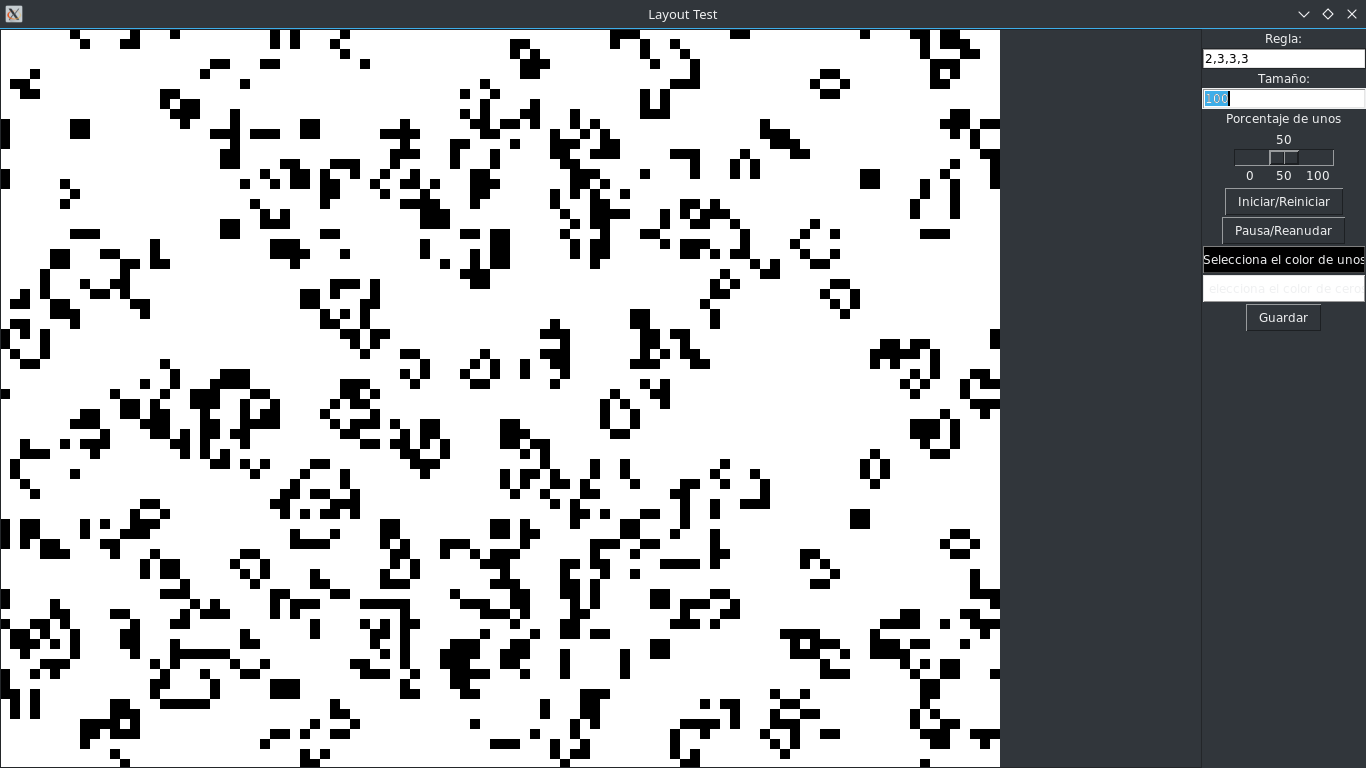
\includegraphics[width=13cm, height=6cm]{./img/gol.png}
 \caption{Juego de la vida con la regla 2333}
 \label{fig:gol}
\end{center}
\end{figure}

\begin{figure}[H]
\begin{center}
 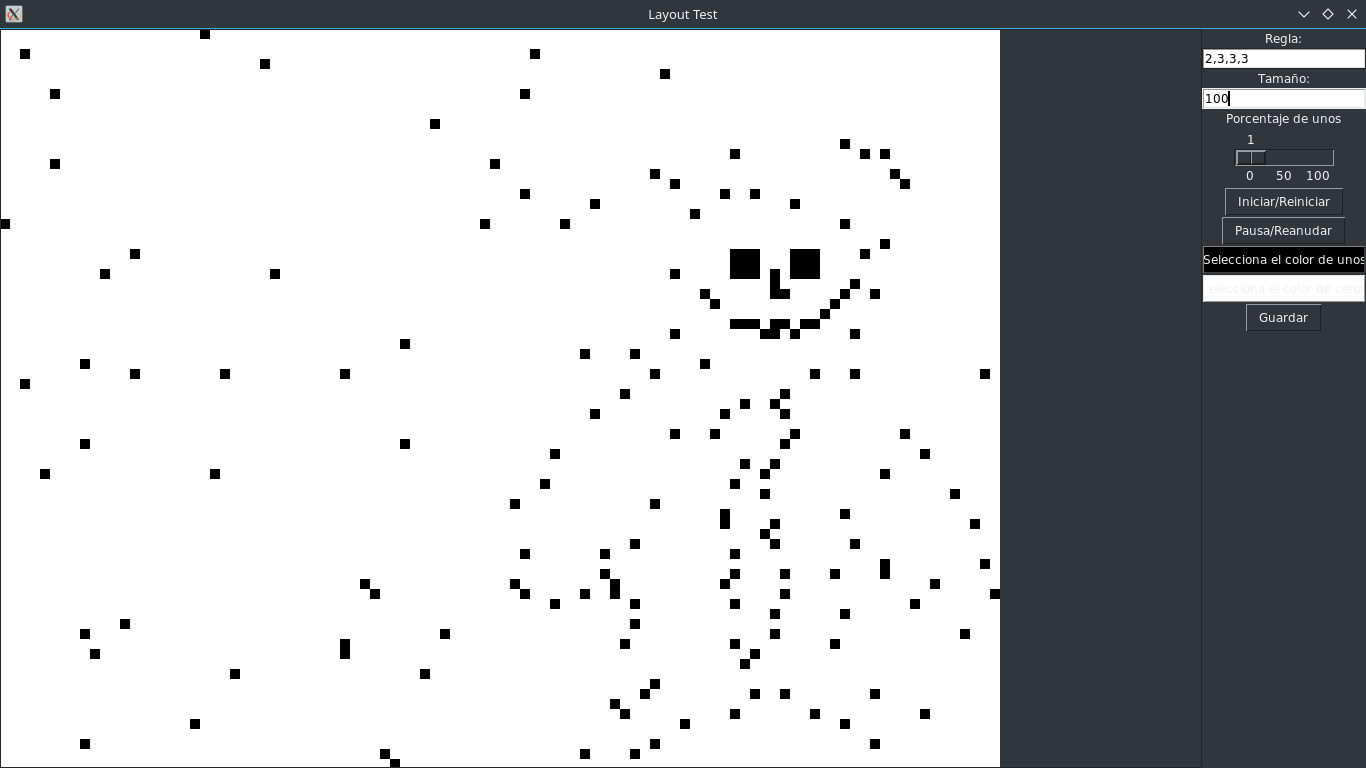
\includegraphics[width=13cm, height=6cm]{./img/gol_celulas.png}
 \caption{Juego de la vida con células seleccionadas por el usuario}
 \label{fig:gol_celulas}
\end{center}
\end{figure}

\begin{figure}[H]
\begin{center}
 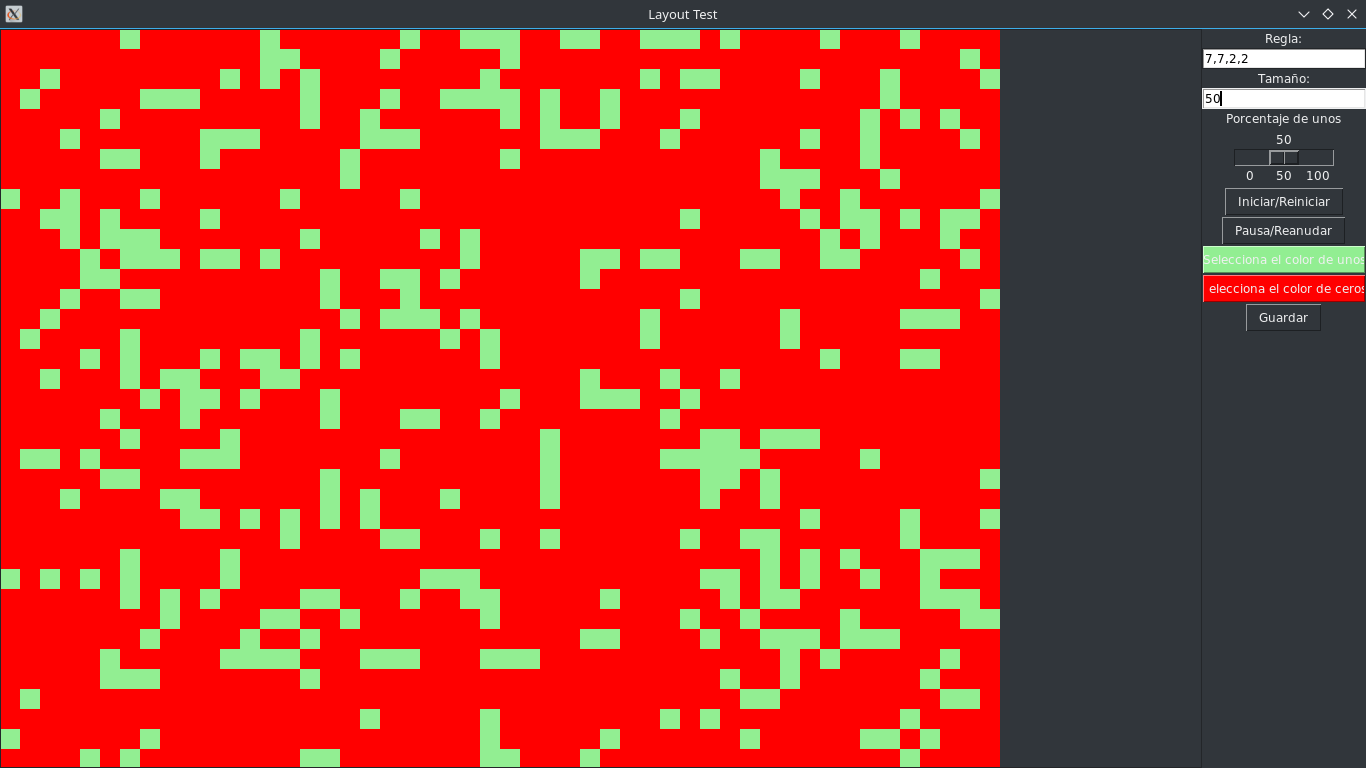
\includegraphics[width=13cm, height=6cm]{./img/gol_colores.png}
 \caption{Juego de la vida cambiando los colores y la regla 7722}
 \label{fig:gol_colores}
\end{center}
\end{figure}

\begin{figure}[H]
\begin{center}
 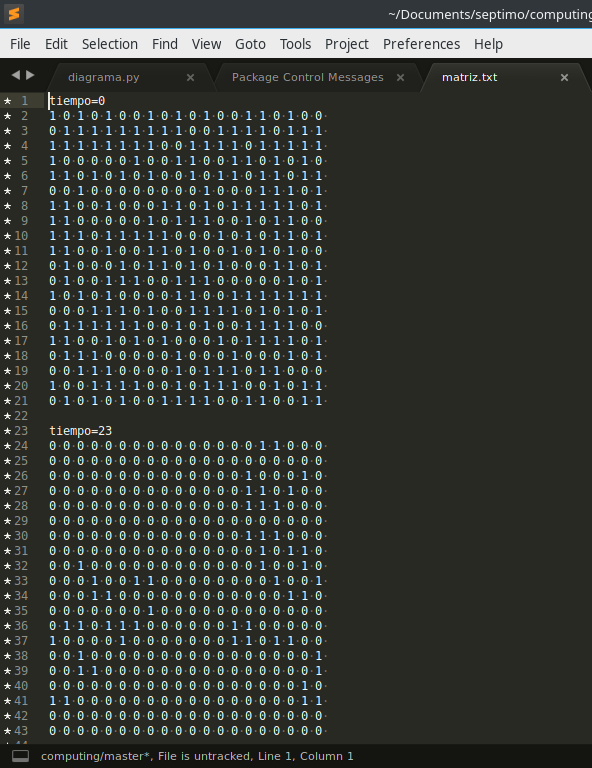
\includegraphics[width=8cm, height=13cm]{./img/matriz.png}
 \caption{Matriz que se guarda}
 \label{fig:matriz}
\end{center}
\end{figure}

\subsubsection{Análisis de poblaciones}
En esta parte se hicieron pruebas con la regla de life y difusión aumentando la densidad de la población de 10 en 10 por ciento hasta llegar al máximo de 100 por ciento, las pruebas de realizaron tras 500 generaciones en una matriz de 100 por 100.

\subsection{Conclusiones}
Al hacer y probar este programa se pudieron solucionar dos cuestiones, la primera es si existe una configuración el la cual el numero de células no se termine, y la respuesta a esto es que exista un oscilador el cual cambia su posición a lo largo del tiempo, otra posible opción es que haya figuras como un bloque formado por 4 cuadros en el cual no hay cambios.

La siguiente cuestión es si existe una configuración en la cual la población crezca indefinidamente. Para lograr esto es indispensable tener un espacio que sea infinito en el cual se puedan propagar las células a través del tiempo, ya que si no se cuenta con esto en algún punto se tendrán tantos elementos vivos que empezaran a morir por sobre población.
